\mysubsection{Ressources}

\ifbook{
  \mysubsubsection{Qu'est ce qu'une ressource ?}
}

\ifslide{
  \begin{frame}{Les ressources}
    \begin{block}{Qu'est ce qu'une ressource ?}
      \begin{itemize}
        \item une base de données (\textit{of course})
        \item un fichier
        \item la ressource désignée par une URL
        \item un fichier dans le classpath !
        \item ...
      \end{itemize}
    \end{block}

    \begin{block}{Caractéristiques}
      \begin{itemize}
        \item externe au processus d'exécution du programme
        \begin{itemize}
          \item un cache local n'est pas, par exemple, une ressource
        \end{itemize}
        \item I/O
        \item doit être gérée:
        \begin{itemize}
          \item fermerture de connection (suivi des connections)
          \item transaction
          \item sécurité
        \end{itemize}
      \end{itemize}
    \end{block}
  \end{frame}

  \begin{frame}
    \begin{block}{\textit{Connection pooling}}
      \begin{itemize}
        \item ouverture de connection couteuse
        \item connections partagées
        \item prêtes à utiliser
      \end{itemize}
    \end{block}
  \end{frame}
}


\ifbook{
  \mysubsubsection{SQL et base de données relationnelle}
}

\ifslide {
  \begin{frame}{Base de donnée relationnelle (SQL)}
    \begin{center}
      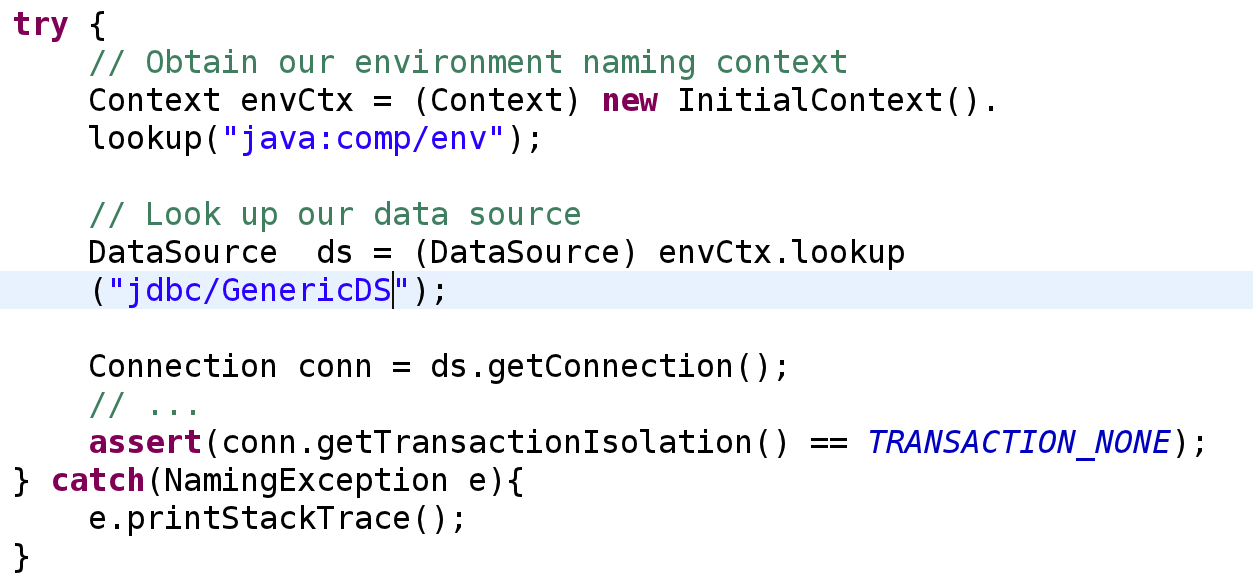
\includegraphics[scale=0.3]{img/datasource-connection.png}
    \end{center}
  \end{frame}

  \begin{frame}{Base de donnée relationnelle (SQL)}
    \begin{center}
      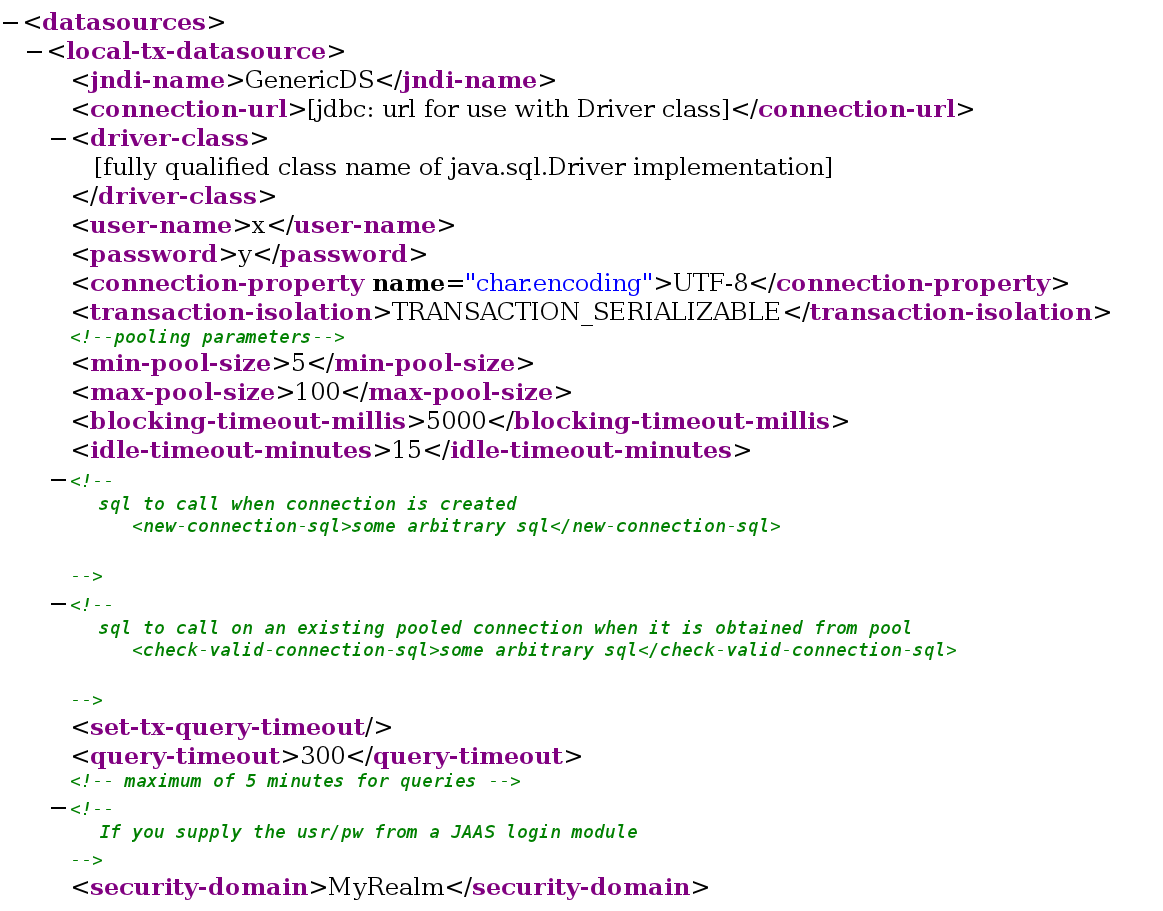
\includegraphics[scale=0.3]{img/datasource.png}
    \end{center}
  \end{frame}

  \begin{frame}{Base de donnée relationnelle (SQL)}
    \begin{block}{Source de données}
      \begin{itemize}
        \item driver
        \item peut être différente d'une base SQL
      \end{itemize}
    \end{block}
  \end{frame}
}

\ifbook{
  \mysubsubsection{Annuaire}
}

\ifslide{
  \begin{frame}{Annuaire (LDAP)}
    \begin{center}
      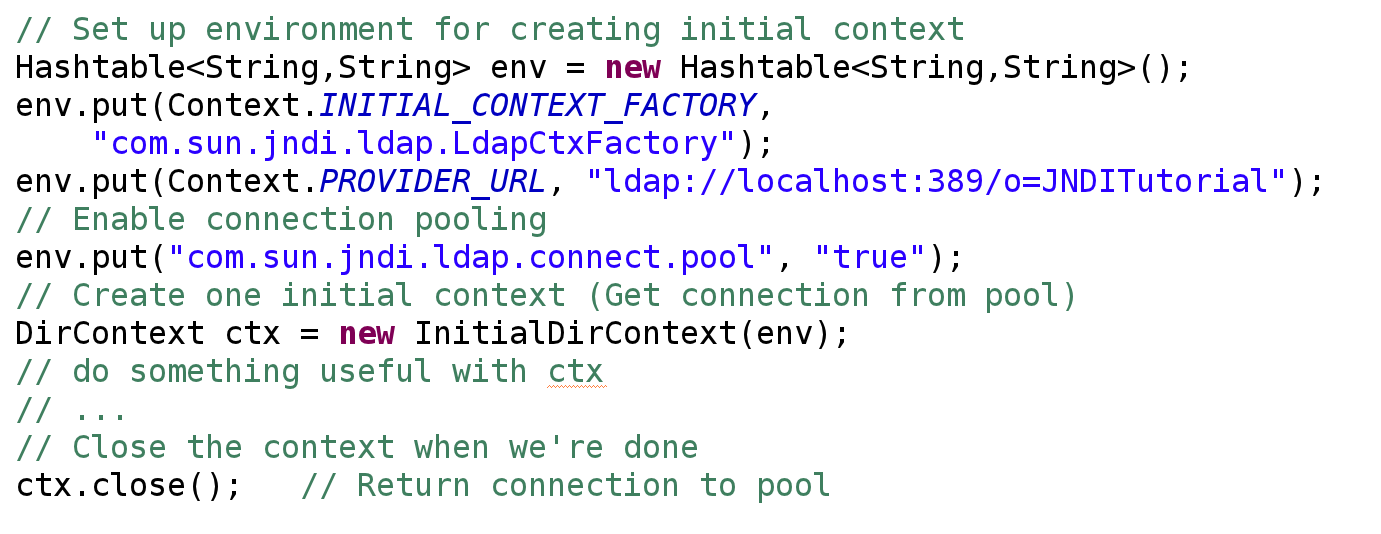
\includegraphics[scale=0.3]{img/ldap-pooling.png}
    \end{center}
  \end{frame}
}

\ifbook{
  \mysubsubsection{NoSQL}
}

\ifslide{
  \begin{frame}{NoSQL}
    \begin{block}{Base NoSQL}
      \begin{itemize}
        \item reste des ressource
        \item plus ou moins configurable
        \item moins standard
        \item plus "sexy"
      \end{itemize}
    \end{block}

    \begin{block}{Fonctionnement}
      \begin{itemize}
        \item clé/valeur (memcached)
        \item document (mongodb)
        \item graphe (neo4j)
        \item objet (db4o)
        \item "hybride" (infinite span)
      \end{itemize}
    \end{block}

  \end{frame}
}
